Many architectures expose the abstraction of virtual memory. While the
implementation of virtual memory is fairly similar across architectures and
operating systems, for concreteness I will use the RISC-V ISA (privileged
architecture version 1.10\cite{riscv_priv110}), and Linux version
4.15\cite{linux} for most examples in this thesis.

With virtual memory, the addresses issued through load and store instructions
do not directly correspond with physical address on the memory bus. Instead,
they are translated to physical addresses through a data structure called the
\gls{pgtbl} (see Figure \ref{fig:generic_paging}).  Page tables contain
translations for fixed-sized ranges of memory called \glspl{page} (\SI{4}{\kibi\byte}
in RISC-V). In addition to translations, each \gls{pte} contains meta-data about the page such as read/write permissions, page
validity, and whether the page has been read or written to recently (called
``accessed'' and ``dirty'' respectively). Throughout this thesis I will refer to
the logical group of data as a ``page'' and the physical region of memory
containing that page as a ``page frame'' or simply ``frame''.  

\begin{figure}[h]
    \centering
    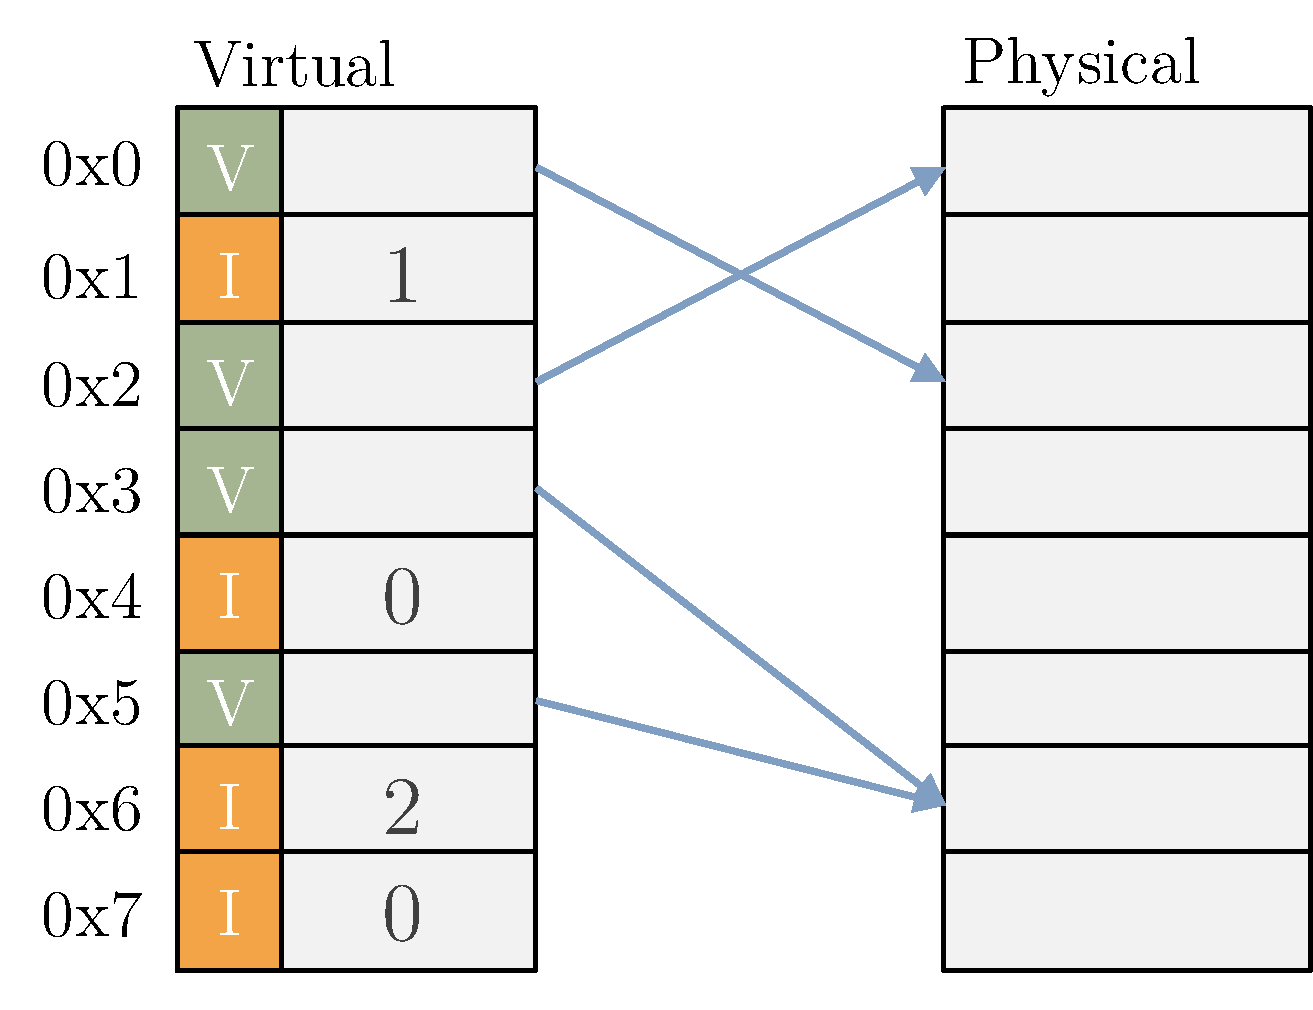
\includegraphics[width=0.5\columnwidth]{figs/generic_page_table.pdf}
    \caption{Example page-table. Entries with a ``V'' are valid (have the valid
             bit set) while ``I'' indicates an invalid entry (valid bit clear).
           Addresses refer to virtual page number (the 52 most significant bits
         in RISC-V).}
    \label{fig:generic_paging}
\end{figure}

Figure \ref{fig:generic_paging_flow} shows a flow chart for translating a page:

\begin{outline}[enumerate]
  \1 The CPU issues a load or store for a particular virtual address
  \1 The load/store unit queries a small cache of recently used translations
  called the \gls{tlb}.
    \2 If the translation is found, a physical address is returned to the CPU
    which then performs the memory access.
  \1 If the translation is not found, the TLB uses a hardware block called the
  \gls{ptw} to find the relevant PTE in main memory.
    \2 If the PTE is marked valid, the physical address is returned to both the
    TLB (for caching) and the CPU.
  \1 If the PTE is marked invalid, the PTW issues a page-fault to the CPU which
  then traps into the OS to handle the invalid memory access.
\end{outline}

\begin{figure}[h]
    \centering
    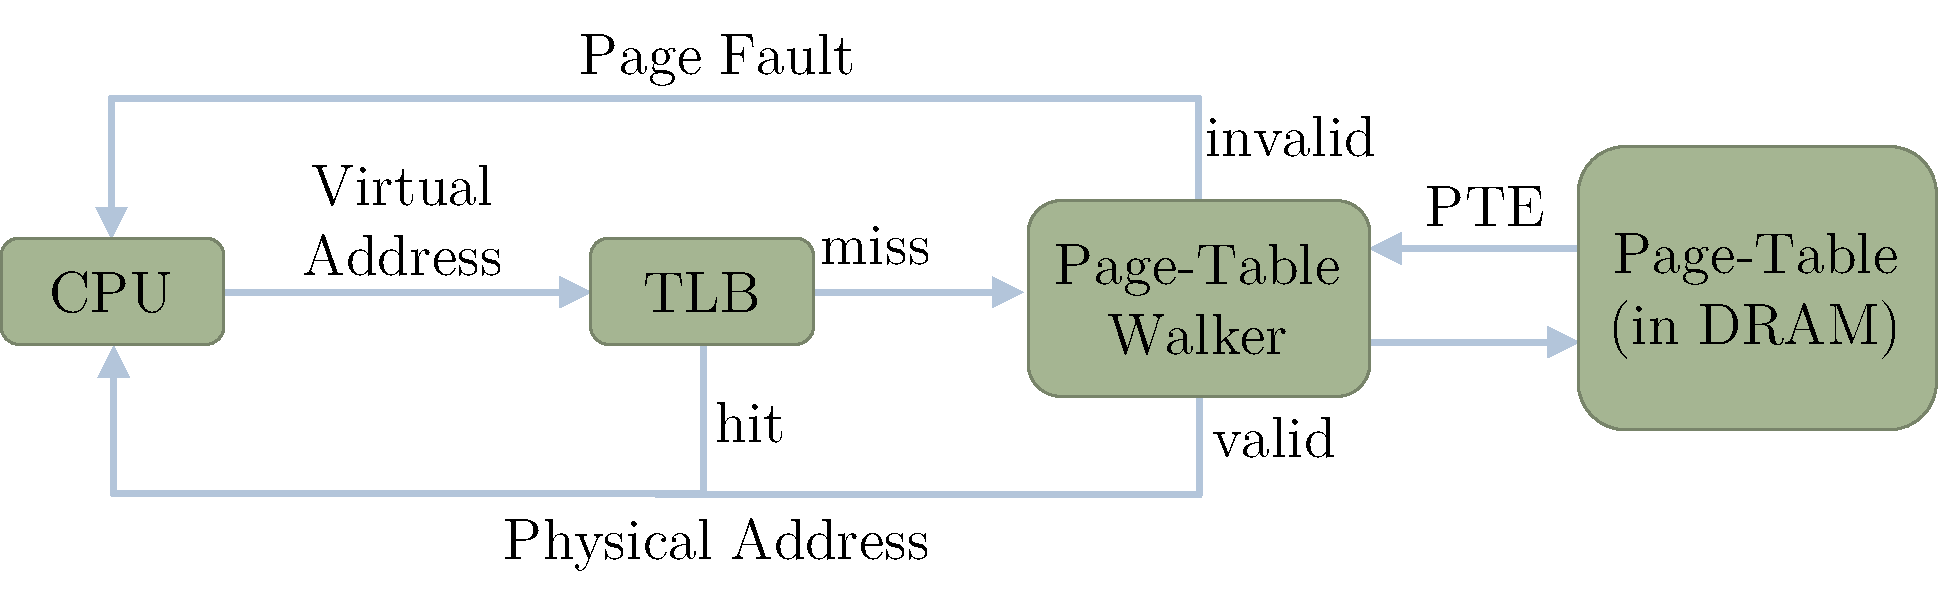
\includegraphics[width=0.9\columnwidth]{figs/generic_paging.pdf}
    \caption{Flow chart for virtual to physical address look up in a typical
      virtual memory system. The translation look aside buffer (TLB) caches
      translations. The page-table walker (PTW) fetches mappings from main
      memory when the TLB misses. Most mappings are valid and can be returned
      directly to the CPU, but invalid mappings result in a trap to the OS.}
    \label{fig:generic_paging_flow}
\end{figure}

In addition to providing memory protection and dirty/accessed tracking, virtual
memory enables a number of operating system techniques to manage physical
memory through the page-fault mechanism. For example, new virtual memory
allocations in Linux do not get physical addresses assigned immediately.
Instead, the OS protects all reads and writes to the page, and only allocates
memory if and when the process actually attempts to use it (virtual address 0x4
in Figure \ref{fig:generic_paging} for example). This saves considerable memory
allocation overheads when processes allocate more memory than they actually use
(a fairly common occurrence). Another technique, called paging, creates the
appearance of unlimited memory by transparently moving pages to an external
storage device (such as a hard disk) and bringing them back only when accessed.
This effectively turns main memory into a software-managed cache for the
external storage device. It does this by marking the evicted pages as
``invalid'', and storing their location on the storage device in the PTE. For
example in Figure \ref{fig:generic_paging}, virtual pages 0x1 and 0x6 are
currently stored on an external storage device at index 1 and 2, respectively.

